\chapter{Background}
\section{Recommender System}
A recommender system is an Information Filtering (IF) system that provides or suggests relevant items to user based on the user profile and preferences. Basic idea of general recommender model is given in : \autoref{fig:recommender_model} \\

\begin{figure}[H]
	\centering
	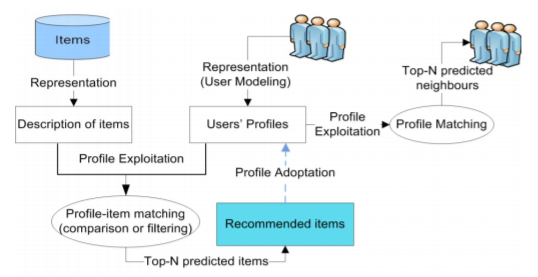
\includegraphics[width=0.7\linewidth]{recommender_model}
	\caption{General Recommender Model \cite{Khusro2016}}
	\label{fig:recommender_model}
\end{figure}

\noindent Traditionally there are two basic models of recommender systems. \begin{itemize} \item Content based filtering \item Collaborative filtering \end{itemize}


\pagebreak

\subsection{Content Based Filtering}
In Content based method algorithm, user preference is considered based on item description. The rating and buying behavior of users are combined with content information available in the items. The main aim of content based filtering is to create profile for each item and each user to find similar items the user is looking for \cite{contentbased}.
\\

\begin{figure}[H]
	\centering
	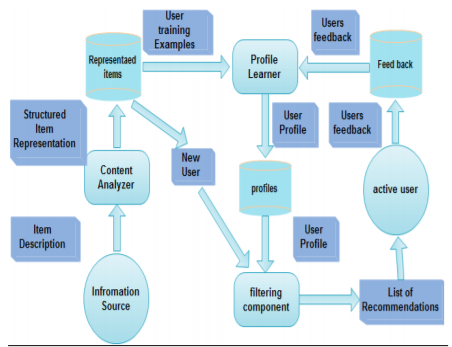
\includegraphics[width=0.7\linewidth]{contentbased_architecture}
	\caption{Content Based filtering Architecture \cite{figures}}
	\label{fig:contentbased_architecture}
\end{figure}

\noindent In this algorithm each user's information can be stored in vector form which contains past behavior of the user. This vector is known as profile vector or user profile. All the information about item is stored in item vector / item profile which contains all the details about item specific attributes. Based on similarity score between user profile and item profile most relevant items are recommended to user. 
\\
Advantages of content-based recommenders are – 
\\
Content-based recommender systems are heavily reliable on the contents of the items that have been rated by the user. So, while making recommendations, this approach would consider user’s taste and accordingly recommend an item that matches user’s preferences. Generally, most popular items dominate less popular items. But this approach will not miss less popular item if it matches the user’s unique taste \cite{contentbased}.
\\
Disadvantages of content-based recommenders
\\
User profiles are generated based on rated items. But for any new user who has not rated any items yet, user profile will be empty. In that case, recommending perfect item that matches to user’s taste is difficult as system does not have user taste information. This problem is known as cold start. Also, to understand each items feature, system needs to examine content of every item. Therefore if number of items rises quickly, performance of the system decreases \cite{contentbased}.  
\\

\subsection{Collaborative Filtering}
Collaborative filtering uses other users’ behavior in the system to predict and recommend items. It depends on user’s contribution such as ratings, reviews which considered as filter for user preference information. The fundamental idea of collaborative filtering is it selects other users’ opinions and aggregate in such way that it provides prediction for active user based on his preferences \cite{CF}. 
\\The main source of input for this algorithm is in the form of matrix of collected user-item ratings. Based on this input it provides recommendations as an output. The first step of output is to predict ratings for items that user may like. Second step is to recommend a list of top rated items as top-N items.
\\

\begin{figure}[H]
	\centering
	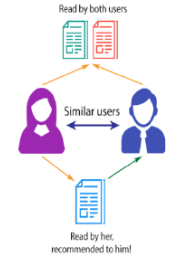
\includegraphics[width=0.7\linewidth]{collaborative_filtering}
	\caption{Collaborative Filtering \cite{cf_figures}}
	\label{fig:collaborative_filtering}
\end{figure}


Collaborative Filtering is broadly divided into 2 categories. 
\\
\subsubsection{Memory-Based (user based)}
A memory-based collaborative filtering approach predicts item ratings based on ratings given by different users for an item. There are primary two forms of memory-based collaborative filtering.
\paragraph{User-User CF:} 
Similarity between users is calculated based on how similarly they rate several items. It finds other users whose ratings are similar to active user and use their ratings on other items to predict what active user may like. Thus it recommends items to the users that are most preferred by similar users.
\\
Consider example of user and ratings given by users to different recipes. This algorithm will find similarity between each user based on the ratings they have given to the recipes in the past. The prediction of a recipe for a user u is calculated by computing weighted sum of the user ratings given by other users to recipe i.
The prediction for recipe I is given as below:
\\
\begin{equation}
P_{u,v} = \frac { \sum_v(r_{v,i} * S_{u,v})}{\sum_v S_{u,v}}
\end{equation}
\\
Where, 
\\
\noindent
$P_{u,i} = $ \text{prediction of recipe } $i$ 
\\
$R_{v,i} = $ \text{rating given by user} $v$ \text{ to recipe } $i$ 
\\
$S_{u,v} = $\text{similarity between users.} 
\\

\noindent To predict the ratings for other user we need to calculate similarity score. The similarity between users can be calculated with the help of several methods described in the section 2.4.3 Prior to that we need to find items rated by both users and its rating. Based on that rating, if we opt to calculate similarities with the Pearson correlation then we will get correlation score between users. Higher correlation implied higher similarity. Recommendations are made based on these prediction values. 
\\
This algorithm is quite expensive in terms of time as it involves calculating similarity score between each user and from that score calculating predictions. This could be very useful when we have less number of users and more items. 
\subsubsection{Model-Based (item based)}


\section{Similarity Methods}
There are several methods available to calculate similarity score.
\\

\subsection{Cosine Similarity}
In this method, cosine of the angle between profile vector and item vector is calculated. Consider A and B are profile vector and item vector respectively, the similarity between them can be calculated as per below formula:
\\

\begin{equation}
sim(A,B) = cos(\theta) =\frac {A.B}{\parallel A \parallel \parallel B \parallel}
\end{equation}

\noindent The value of cosine angle ranges between -1 to 1. Lesser the angle, less distance hence more similarity as cos(0) = 1. Then items are arranged in descending order and recommended to user
\\
\subsection{Euclidean Distance}
If we plot similar items in n-dimensional space, then they will fall under close proximity. In that case, we can calculate distance between items with Euclidean distance formula which is given by:
\\
\begin{equation}
Euclidean Distance = \sqrt{(x_1 - y_1)^2 + ... + (x_n - y_n)^2}
\end{equation}


\subsection{Pearson’s Correlation}
Person’s correlation helps in finding correlation between similar items. Correlation on higher side implies more similarity. It can be calculated as below:
\\
\begin{equation}
sim(u,v) = \frac{\sum (r_{ui} - \bar{r}_u) (r_{vi} - \bar{r}_v )}{\sqrt{(\sum (r_{ui} - \bar{r}_u))^2} \sqrt{(\sum (r_{vi} - \bar{r}_v )^2}}
\end{equation}
\\